\section{Introduction}
Neural radiance fields made photorealistic novel-view synthesis possible, but their volumetric evaluation is expensive~\cite{mildenhall2020nerf,barron2021mipnerf,muller2022instant,chen2022tensorf}. 3D Gaussian Splatting (3DGS) replaces repeated network queries with an explicit set of anisotropic Gaussians and a differentiable tile rasterizer, yielding high quality and real-time rendering~\cite{kerbl2023gaussians}. Its efficiency at inference, however, does not make training memory-free. Adaptive density control repeatedly clones and splits primitives; parameters, gradients, optimizer moments, temporary concatenations, and rasterization buffers coexist during mutation.

This distinction matters on consumer GPUs. A fixed Gaussian-count cap ignores the different transient costs of cloning and splitting and the current state of the caching allocator. Conversely, frequent opacity or utility pruning can be counterproductive: a new Gaussian often begins with weak opacity and incomplete view support, so a policy that applies hygiene eviction at every density-control cycle can remove it before optimization establishes its value. We call this the \emph{over-pruning dilemma}: freeing memory early may prevent the representation from reaching a useful spatial allocation.

We study the problem under an explicit peak-memory operating envelope rather than post-training model compression. Figure~\ref{fig:framework} summarizes \method. The system estimates current headroom from allocated and reserved CUDA memory, adds a non-PyTorch allowance, predicts affine clone/split costs, and admits a feasible mutation batch. Within that batch, a greedy gain-per-byte allocator prioritizes spatial demand. The main empirical finding is that the lifecycle policy dominates the inflow schedule: retaining low-scored Gaussians when headroom is sufficient, and pruning them only under admission pressure, produces much higher reconstruction quality than unconditional hygiene pruning in the evaluated implementation.

\begin{figure*}[t]
  \centering
  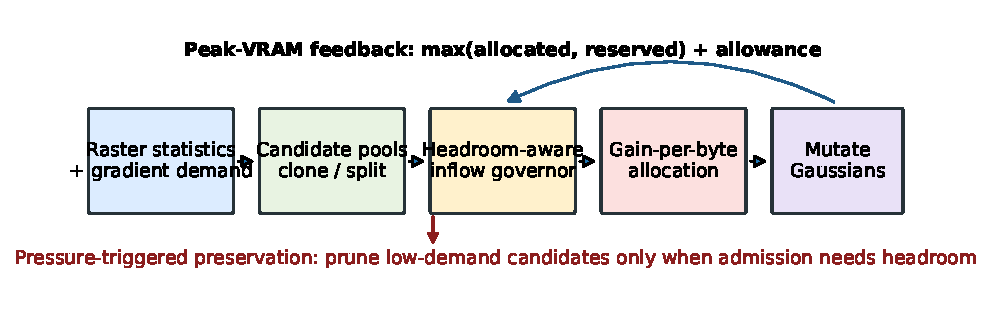
\includegraphics[width=\textwidth]{figures/fig1_framework.pdf}
  \caption{\method closes the loop between raster-derived spatial demand and allocator headroom. Pressure-triggered preservation is an admission-dependent lifecycle rule, not a post-training compression stage.}
  \label{fig:framework}
\end{figure*}

Our contributions are:
\begin{itemize}
  \item a peak-VRAM-aware mutation controller with calibrated affine clone/split costs and a dynamic 5K--15K inflow policy;
  \item a pressure-triggered preservation lifecycle that couples eviction to actual headroom demand, avoiding eager removal of under-optimized primitives;
  \item a complete 2x2 inflow-by-lifecycle ablation, three-seed paired validation on Bonsai, and single-seed evaluation on two additional Mip-NeRF 360 scenes;
  \item an evidence-traceable memory study that separates controller footprint from sampled whole-device VRAM and limits the claim to empirical boundedness.
\end{itemize}
